%%%%%%%%%%%%%%%%%%%%%%%%%%%%%%%%%%%%%%%%%
% Beamer Presentation
% LaTeX Template
% Version 2.0 (March 8, 2022)
%
% This template originates from:
% https://www.LaTeXTemplates.com
%
% Author:
% Vel (vel@latextemplates.com)
%
% License:
% CC BY-NC-SA 4.0 (https://creativecommons.org/licenses/by-nc-sa/4.0/)
%
%%%%%%%%%%%%%%%%%%%%%%%%%%%%%%%%%%%%%%%%%

%----------------------------------------------------------------------------------------
%	PACKAGES AND OTHER DOCUMENT CONFIGURATIONS
%----------------------------------------------------------------------------------------

\documentclass[
	10pt, % Set the default font size, options include: 8pt, 9pt, 10pt, 11pt, 12pt, 14pt, 17pt, 20pt
	%t, % Uncomment to vertically align all slide content to the top of the slide, rather than the default centered
	%aspectratio=169, % Uncomment to set the aspect ratio to a 16:9 ratio which matches the aspect ratio of 1080p and 4K screens and projectors
]{beamer}

\graphicspath{{figures/}{./}} % Specifies where to look for included images (trailing slash required)


\usepackage{booktabs} % Allows the use of \toprule, \midrule and \bottomrule for better rules in tables
\usepackage{multimedia}
\usepackage{hyperref}
\usepackage{outlines}
\usepackage{float}
% \usepackage{caption}
\usepackage{subcaption}
\usepackage{cases}
%----------------------------------------------------------------------------------------
%	SELECT LAYOUT THEME
%----------------------------------------------------------------------------------------

% Beamer comes with a number of default layout themes which change the colors and layouts of slides. Below is a list of all themes available, uncomment each in turn to see what they look like.

%\usetheme{default}
%\usetheme{AnnArbor}
%\usetheme{Antibes}
%\usetheme{Bergen}
%\usetheme{Berkeley}
%\usetheme{Berlin}
%\usetheme{Boadilla}
%\usetheme{CambridgeUS}
% \usetheme{Copenhagen}
%\usetheme{Darmstadt}
%\usetheme{Dresden}
%\usetheme{Frankfurt}
%\usetheme{Goettingen}
%\usetheme{Hannover}
%\usetheme{Ilmenau}
%\usetheme{JuanLesPins}
%\usetheme{Luebeck}
\usetheme{Madrid}
%\usetheme{Malmoe}
%\usetheme{Marburg}
%\usetheme{Montpellier}
%\usetheme{PaloAlto}
%\usetheme{Pittsburgh}
%\usetheme{Rochester}
%\usetheme{Singapore}
%\usetheme{Szeged}
%\usetheme{Warsaw}

%----------------------------------------------------------------------------------------
%	SELECT COLOR THEME
%----------------------------------------------------------------------------------------

% Beamer comes with a number of color themes that can be applied to any layout theme to change its colors. Uncomment each of these in turn to see how they change the colors of your selected layout theme.

% \usecolortheme{albatross}
%\usecolortheme{beaver}
%\usecolortheme{beetle}
%\usecolortheme{crane}
%\usecolortheme{dolphin}
%\usecolortheme{dove}
%\usecolortheme{fly}
%\usecolortheme{lily}
%\usecolortheme{monarca}
%\usecolortheme{seagull}
%\usecolortheme{seahorse}
\usecolortheme{spruce}
%\usecolortheme{whale}
% \usecolortheme{wolverine}

%----------------------------------------------------------------------------------------
%	SELECT FONT THEME & FONTS
%----------------------------------------------------------------------------------------

% Beamer comes with several font themes to easily change the fonts used in various parts of the presentation. Review the comments beside each one to decide if you would like to use it. Note that additional options can be specified for several of these font themes, consult the beamer documentation for more information.

\usefonttheme{default} % Typeset using the default sans serif font
%\usefonttheme{serif} % Typeset using the default serif font (make sure a sans font isn't being set as the default font if you use this option!)
%\usefonttheme{structurebold} % Typeset important structure text (titles, headlines, footlines, sidebar, etc) in bold
%\usefonttheme{structureitalicserif} % Typeset important structure text (titles, headlines, footlines, sidebar, etc) in italic serif
%\usefonttheme{structuresmallcapsserif} % Typeset important structure text (titles, headlines, footlines, sidebar, etc) in small caps serif

%------------------------------------------------

%\usepackage{mathptmx} % Use the Times font for serif text
\usepackage{palatino} % Use the Palatino font for serif text

%\usepackage{helvet} % Use the Helvetica font for sans serif text
\usepackage[default]{opensans} % Use the Open Sans font for sans serif text
%\usepackage[default]{FiraSans} % Use the Fira Sans font for sans serif text
%\usepackage[default]{lato} % Use the Lato font for sans serif text

%----------------------------------------------------------------------------------------
%	SELECT INNER THEME
%----------------------------------------------------------------------------------------

% Inner themes change the styling of internal slide elements, for example: bullet points, blocks, bibliography entries, title pages, theorems, etc. Uncomment each theme in turn to see what changes it makes to your presentation.

%\useinnertheme{default}
\useinnertheme{circles}
%\useinnertheme{rectangles}
%\useinnertheme{rounded}
%\useinnertheme{inmargin}

%----------------------------------------------------------------------------------------
%	SELECT OUTER THEME
%----------------------------------------------------------------------------------------

% Outer themes change the overall layout of slides, such as: header and footer lines, sidebars and slide titles. Uncomment each theme in turn to see what changes it makes to your presentation.

%\useoutertheme{default}
%\useoutertheme{infolines}
%\useoutertheme{miniframes}
%\useoutertheme{smoothbars}
%\useoutertheme{sidebar}
%\useoutertheme{split}
%\useoutertheme{shadow}
%\useoutertheme{tree}
%\useoutertheme{smoothtree}

%\setbeamertemplate{footline} % Uncomment this line to remove the footer line in all slides
%\setbeamertemplate{footline}[page number] % Uncomment this line to replace the footer line in all slides with a simple slide count

%\setbeamertemplate{navigation symbols}{} % Uncomment this line to remove the navigation symbols from the bottom of all slides

%----------------------------------------------------------------------------------------
%	PRESENTATION INFORMATION
%----------------------------------------------------------------------------------------

\title[PhD Interview - ETH Zürich]{PhD Interview - ETH Zürich} % The short title in the optional parameter appears at the bottom of every slide, the full title in the main parameter is only on the title page

\subtitle{Multiphase Modeling of Alpine Mass Movements \\ and Process Cascades} 

\author[Mikkel Metzsch Jensen]{Mikkel Metzsch Jensen} % Presenter name(s), the optional parameter can contain a shortened version to appear on the bottom of every slide, while the main parameter will appear on the title slide

\institute[UiO]{University of Oslo} % Your institution, the optional parameter can be used for the institution shorthand and will appear on the bottom of every slide after author names, while the required parameter is used on the title slide and can include your email address or additional information on separate lines

\date[February 13, 2023]
{February 13, 2023 \\
\vspace*{20px}
\begin{enumerate}
	\item Introduction 
	\item Master's thesis
	\item PhD project interpretation
\end{enumerate}} 



%----------------------------------------------------------------------------------------

\begin{document}

%----------------------------------------------------------------------------------------
%	TITLE SLIDE
%----------------------------------------------------------------------------------------

\begin{frame}
	\titlepage % Output the title slide, automatically created using the text entered in the PRESENTATION INFORMATION block above
\end{frame}

%----------------------------------------------------------------------------------------
%	TABLE OF CONTENTS SLIDE
%----------------------------------------------------------------------------------------

% The table of contents outputs the sections and subsections that appear in your presentation, specified with the standard \section and \subsection commands. You may either display all sections and subsections on one slide with \tableofcontents, or display each section at a time on subsequent slides with \tableofcontents[pausesections]. The latter is useful if you want to step through each section and mention what you will discuss.

% \begin{frame}
% 	\frametitle{Presentation Overview} % Slide title, remove this command for no title
	
% 	\tableofcontents % Output the table of contents (all sections on one slide)
% 	%\tableofcontents[pausesections] % Output the table of contents (break sections up across separate slides)
% \end{frame}

%----------------------------------------------------------------------------------------
%	PRESENTATION BODY SLIDES
%----------------------------------------------------------------------------------------


\section{Introduction}

\begin{frame}
	\frametitle{Academic Background}

	{\large Education}
	\begin{itemize}
		\item Bachelor in Physcis
		\item Master in Computational Science: Materials Science 
	\end{itemize}
	\vspace{0.3cm}
	
	{\large Scientiffic interests}
	\begin{itemize}
		\item Numerical modelling
		\item Optimization problems
		\item Materials science and statistical mechanics
		\item Machine learning
		\item Design and innovation
	\end{itemize}
	\vspace{0.3cm}

	{\large Project priorities - 80,000 hours}
	\begin{enumerate}
		\item Method
		\item Field of application 
		\item Positive impact 
	\end{enumerate}
\end{frame}

\begin{frame}
	\frametitle{Programming experience}
	{\large High level}
	\begin{itemize}
		\item Python
		\item Julia
		\begin{itemize}
			\item More efficient alternative to python
		\end{itemize}
	\end{itemize} 
	\vspace{0.2cm}
	
	{\large Low level}
	\begin{itemize}
		\item C / C++
		\begin{itemize}
			\item High performance computing (HPC)
		\end{itemize}
	\end{itemize}
	\vspace{0.2cm}

	{\large Function based / Modules}
	\begin{itemize}
		\item LAMMPS
		\begin{itemize}
			\item Efficeint workflow for MD simulations
		\end{itemize}
		\item PyTorch / TensorFlow
		\begin{itemize}
			\item Machine learning platforms
		\end{itemize}
	\end{itemize}

\end{frame}


% \begin{frame}
% 	\frametitle{Hobbies and personal interest}
% 	\begin{columns}
% 	\begin{column}{0.6\textwidth}
% 		\vspace{0.5cm}

% 		\begin{itemize}
% 			\item Handstands and ``movement''
% 			\item Skiing (5 years as ski instructor)
% 			\item Hiking 
% 			\item Photography
% 		\end{itemize}
% 		\vspace{0.5cm}


% 		\begin{figure}
% 			\centering
% 			\begin{subfigure}[b]{0.49\textwidth}
% 				\centering
% 				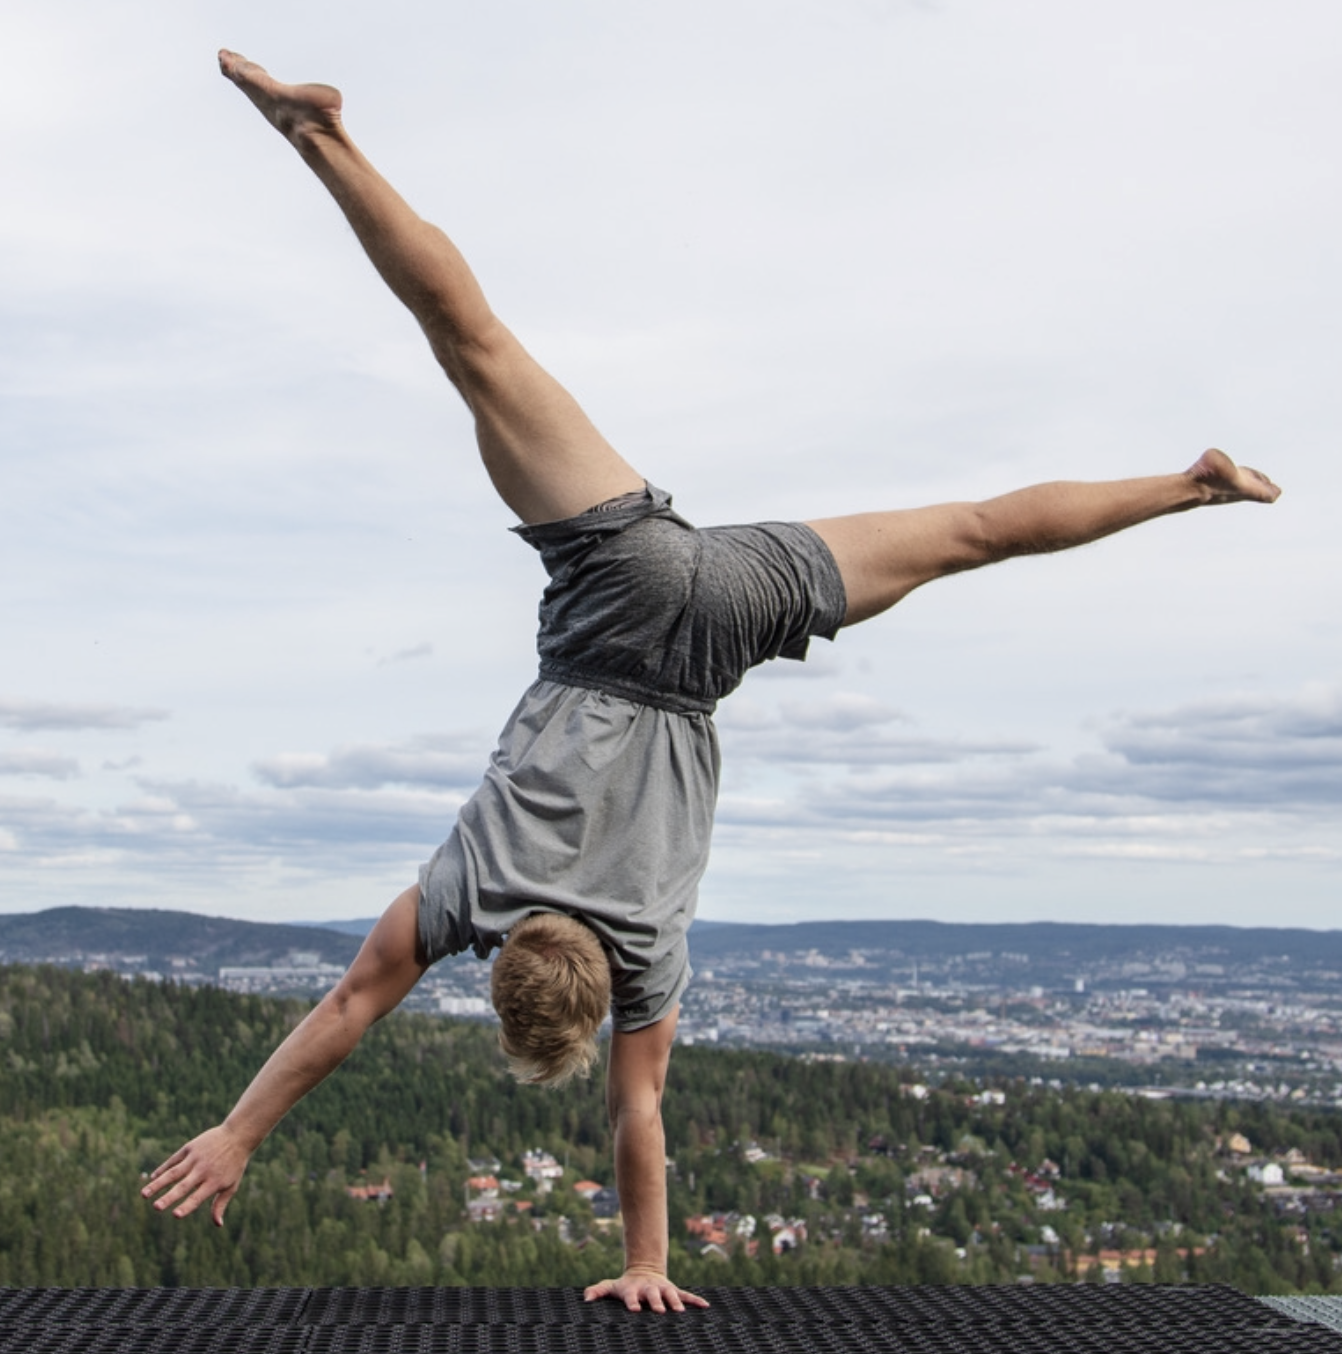
\includegraphics[width=0.38\textheight]{figures/handstand.png}
% 				% \caption{}
% 			\end{subfigure}
% 			\hfill
% 			\begin{subfigure}[b]{0.49\textwidth}
% 				\centering
% 				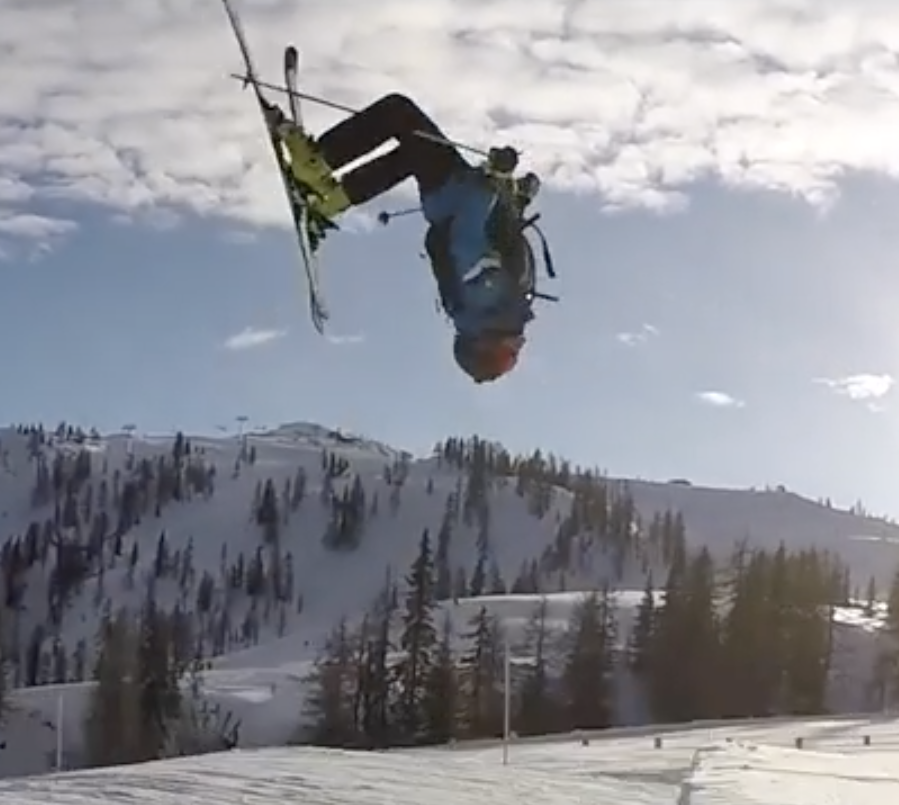
\includegraphics[width=0.43\textheight]{figures/backflip.png}
% 				% \caption{}
% 			\end{subfigure}
% 			%    \caption{}
% 		  \end{figure}

% 	\end{column}



% 	\begin{column}{0.4\textwidth}  

% 		\begin{figure}
% 			\centering
% 			\begin{subfigure}[b]{0.49\textheight}
% 				\centering
% 				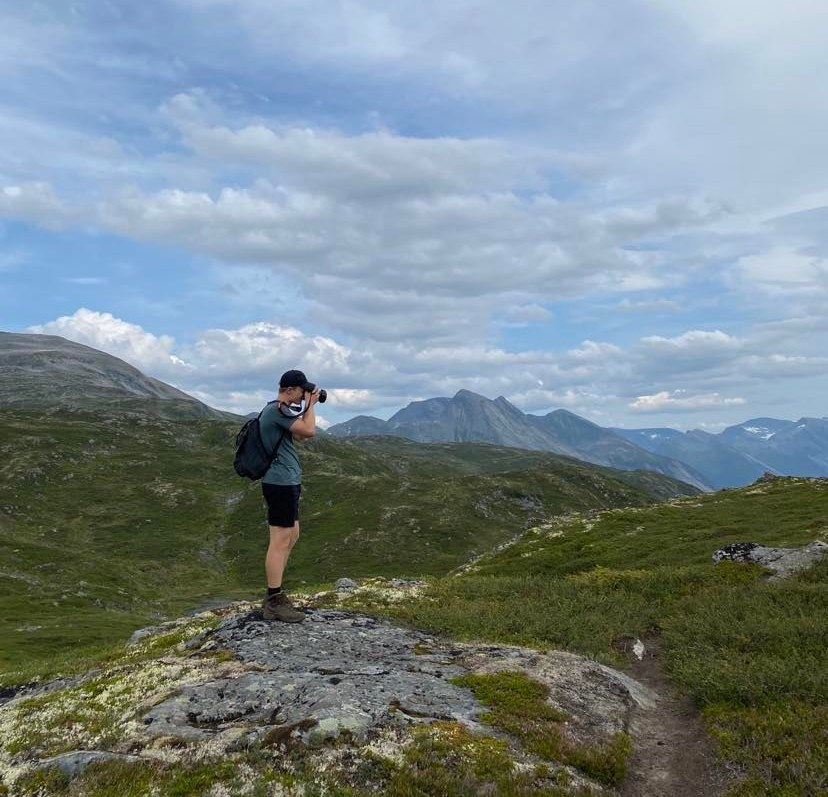
\includegraphics[width=0.4\textheight]{figures/photography.jpg}
% 				% \caption{}
% 			\end{subfigure}
% 			\hfill
% 			\begin{subfigure}[b]{0.49\textheight}
% 				\centering
% 				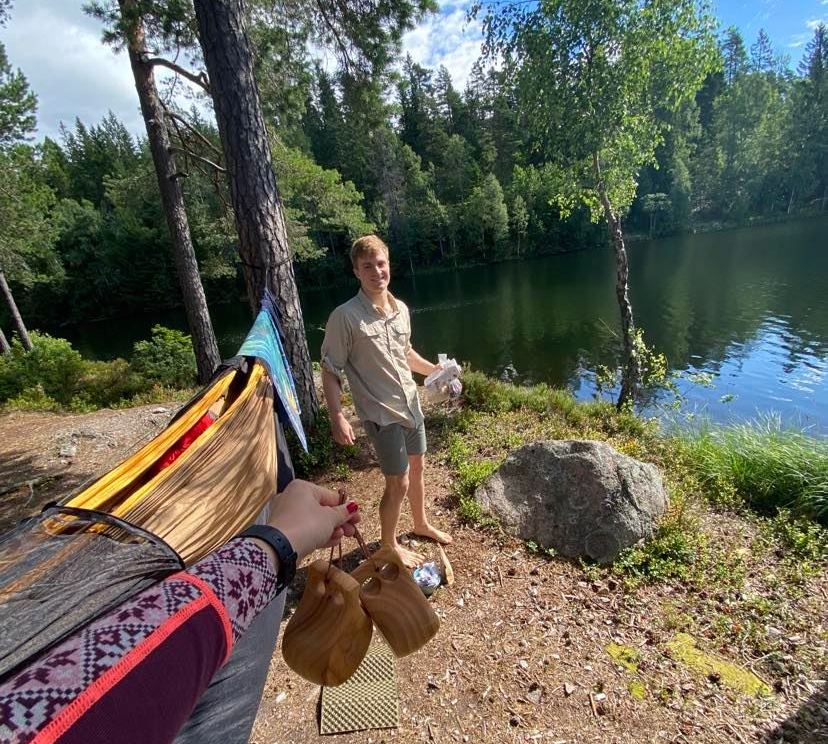
\includegraphics[width=0.4\textheight]{figures/camping.jpg}
% 				% \caption{}
% 			\end{subfigure}
% 			%    \caption{}
% 		  \end{figure}


% 		% \begin{center}
% 		%  %%%%% this is a minipage, so \textwidth is already adjusted to the size of the column
% 		%  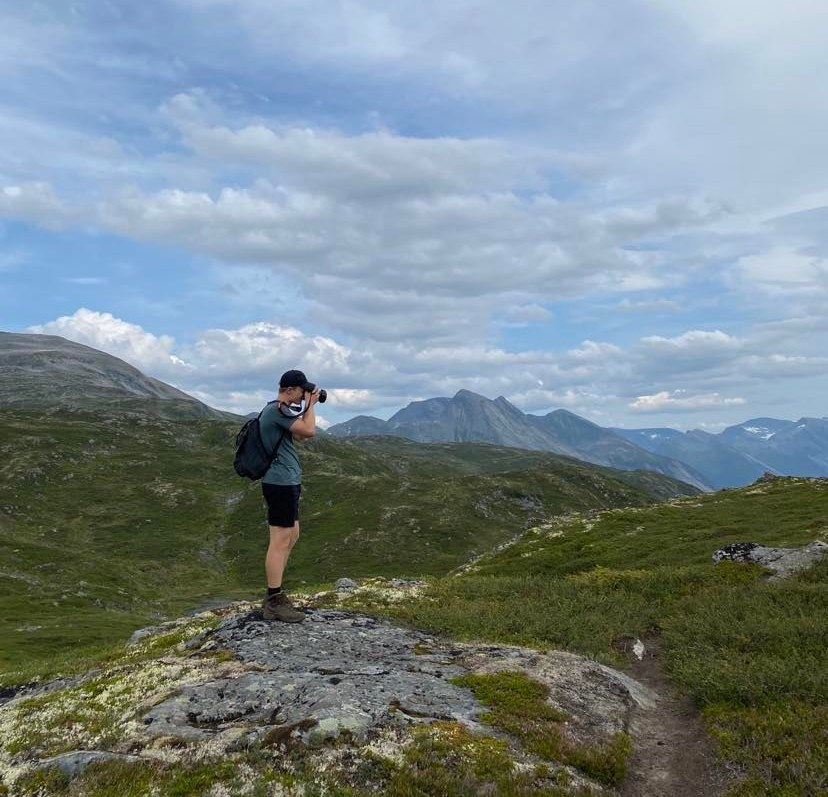
\includegraphics[width=0.7\textwidth]{figures/photography.jpg}
% 		%  \end{center}
% 		% \begin{center}
% 		%  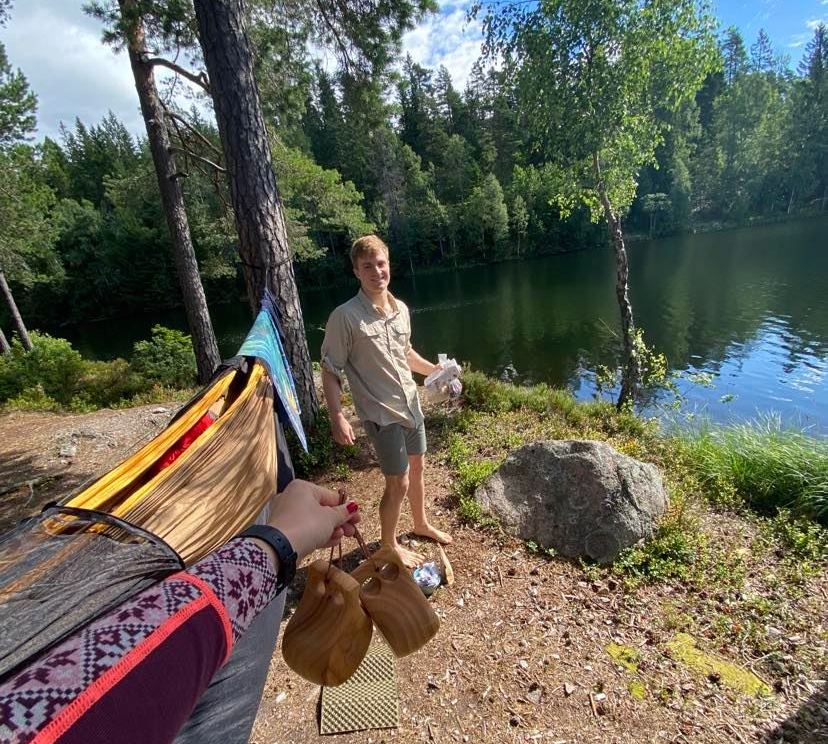
\includegraphics[width=0.7\textwidth]{figures/camping.jpg}
% 		%  \end{center}
% 	\end{column}
% 	\end{columns}
% 	\end{frame}


	\begin{frame}
		\frametitle{Hobbies and personal interests}
		\begin{columns}

		\column{0.6\textwidth}
		\begin{minipage}[c][0.4\textheight][c]{\linewidth}
		\vspace{1cm}
		\begin{itemize}
			\item Handstands and ``movement''
			\item Skiing (5 years as ski instructor)
			\item Hiking / Outdoor 
			\item Photography
		\end{itemize}

		\end{minipage}
	
		\begin{minipage}[c][0.5\textheight][c]{\linewidth}
			% \centering
			% \includegraphics[width=0.8\linewidth]{example-image-c}
			\begin{figure}
				\centering
				\begin{subfigure}[b]{0.49\linewidth}
					\centering
					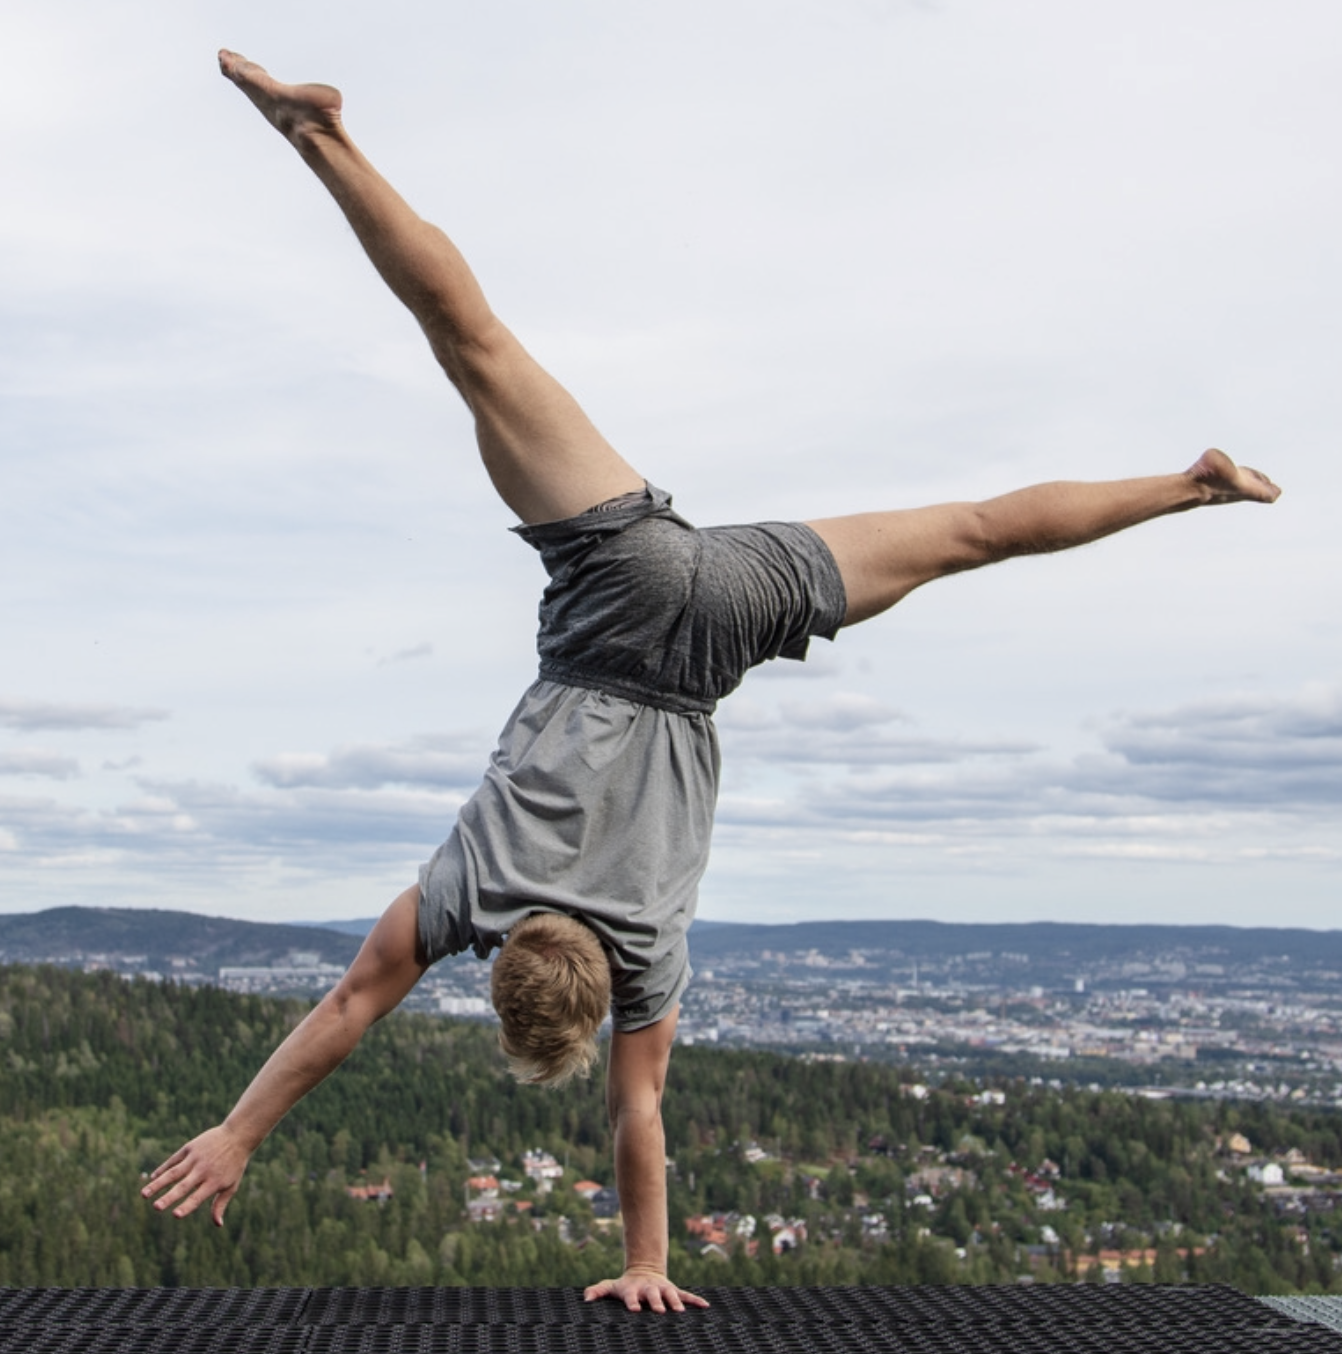
\includegraphics[width=0.355\textheight]{figures/handstand.png}
				\end{subfigure}
				\hfill
				\begin{subfigure}[b]{0.49\linewidth}
					\centering
					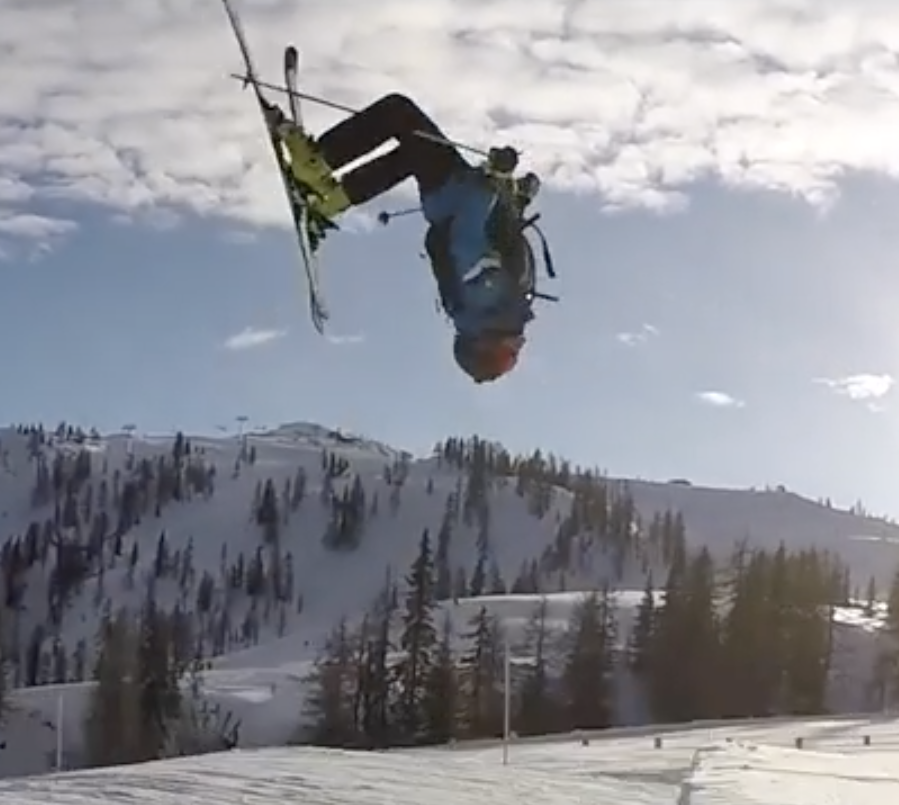
\includegraphics[width=0.4\textheight]{figures/backflip.png}
				\end{subfigure}
			\end{figure}
		\end{minipage}
			
		\column{0.4\textwidth}	
		\begin{minipage}[c][0.4\textheight][c]{\linewidth}
		  \centering  
		  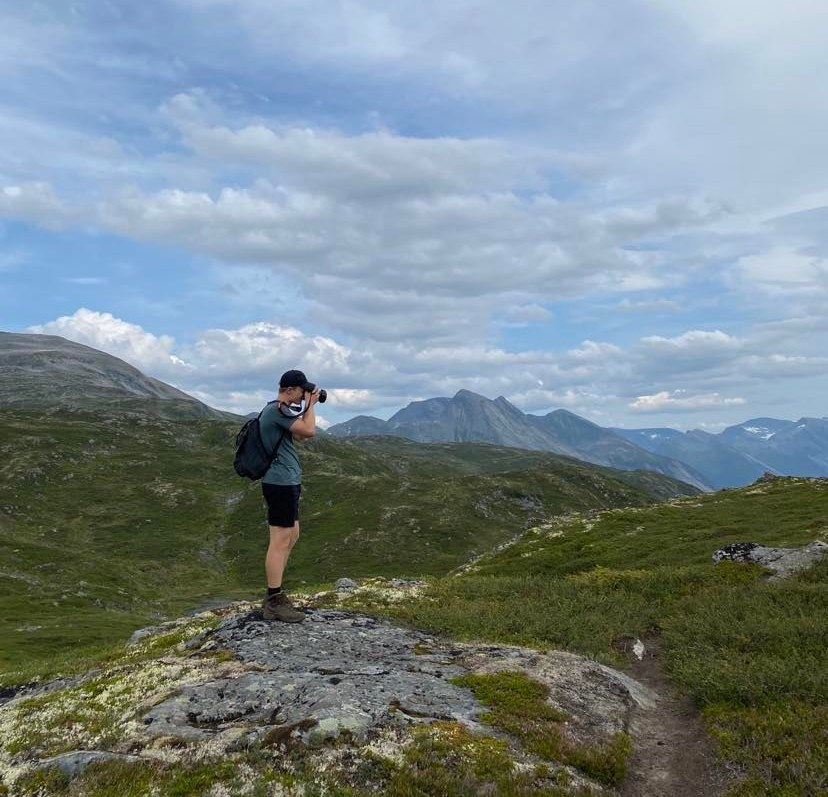
\includegraphics[width=0.75\linewidth]{figures/photography.jpg}
		\end{minipage}  
		\begin{minipage}[c][0.4\textheight][c]{\linewidth}
		  \centering  
		  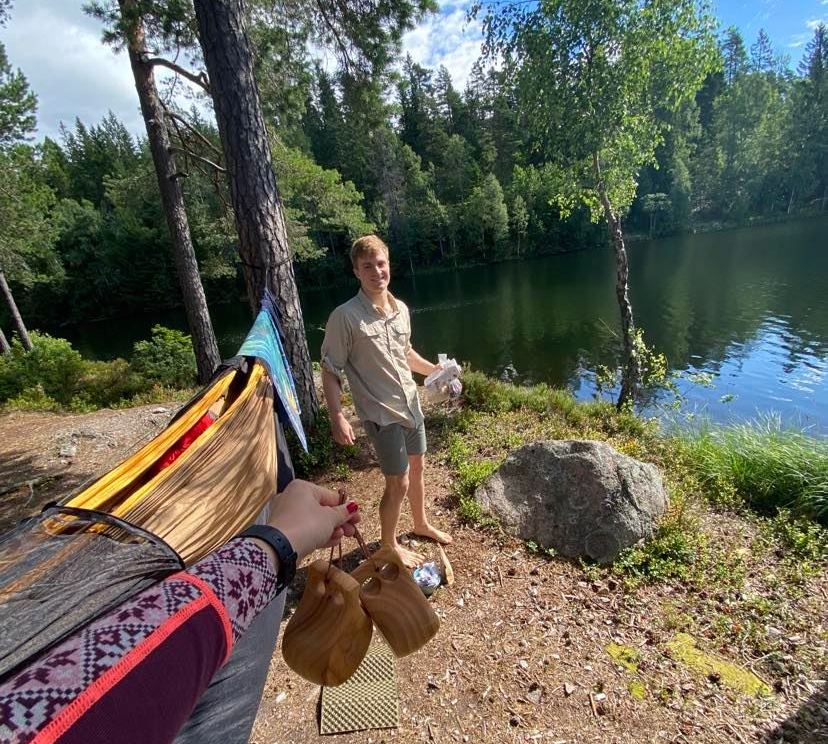
\includegraphics[width=0.75\linewidth]{figures/camping.jpg}
		\end{minipage}  



		\end{columns}
		\end{frame}
		
\section{Master's thesis}


\begin{frame}
	\frametitle{Master's thesis}
	\framesubtitle{3 Phases}

	{\large Tuning frictional properties of graphene sheets using kirigami inspired cuts and inverse design}
	\newline
	
	\begin{enumerate}
		\setlength\itemsep{2em}
		\item \underline{Sheet kirigami}: Alter graphene sheet using atomic scale cuts % Buckling in the 3rd dimension
		\item \underline{Forward simulation}: Calculate frictional properties of the sheet using MD simulations
		\item \underline{Inverse design}: Predict cut patterns based on frictional properties and optimize for desired properties using machine learning
		\begin{itemize}
			\item Low/high friction coefficient
			\item Coupling between stretch and friction
			\item Negative friction coefficients
		\end{itemize} 
	\end{enumerate}
\end{frame}



\begin{frame}
	\frametitle{Motivation}

	\begin{itemize}
		\item Kirigami: Variation of origami with cuts permitted
		\item Macroscale $\to$ Nanoscale
	\end{itemize}
	\vspace*{10px}

	\begin{figure}
		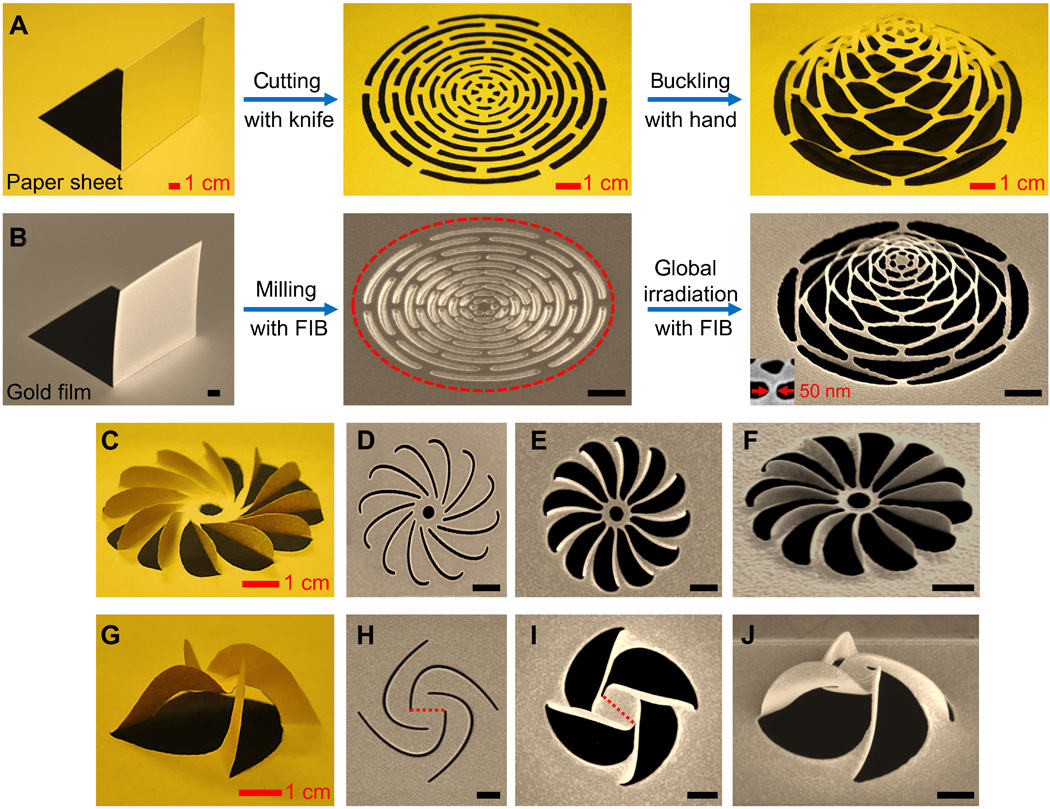
\includegraphics[height=0.6\textheight]{figures/kirigami_example.jpeg}
		\caption{Example of transistion from macro- to nano-kirigami using a focused ion-beam (FIB) (Nano-kirigami with giant optical chirality, ZHIGUANG LIU, 2018).}
	\end{figure}	

\end{frame}

\begin{frame}
	\frametitle{Stage 1 - Sheet Kirigami}
	\framesubtitle{Choosing a cut pattern}

	\begin{figure}
		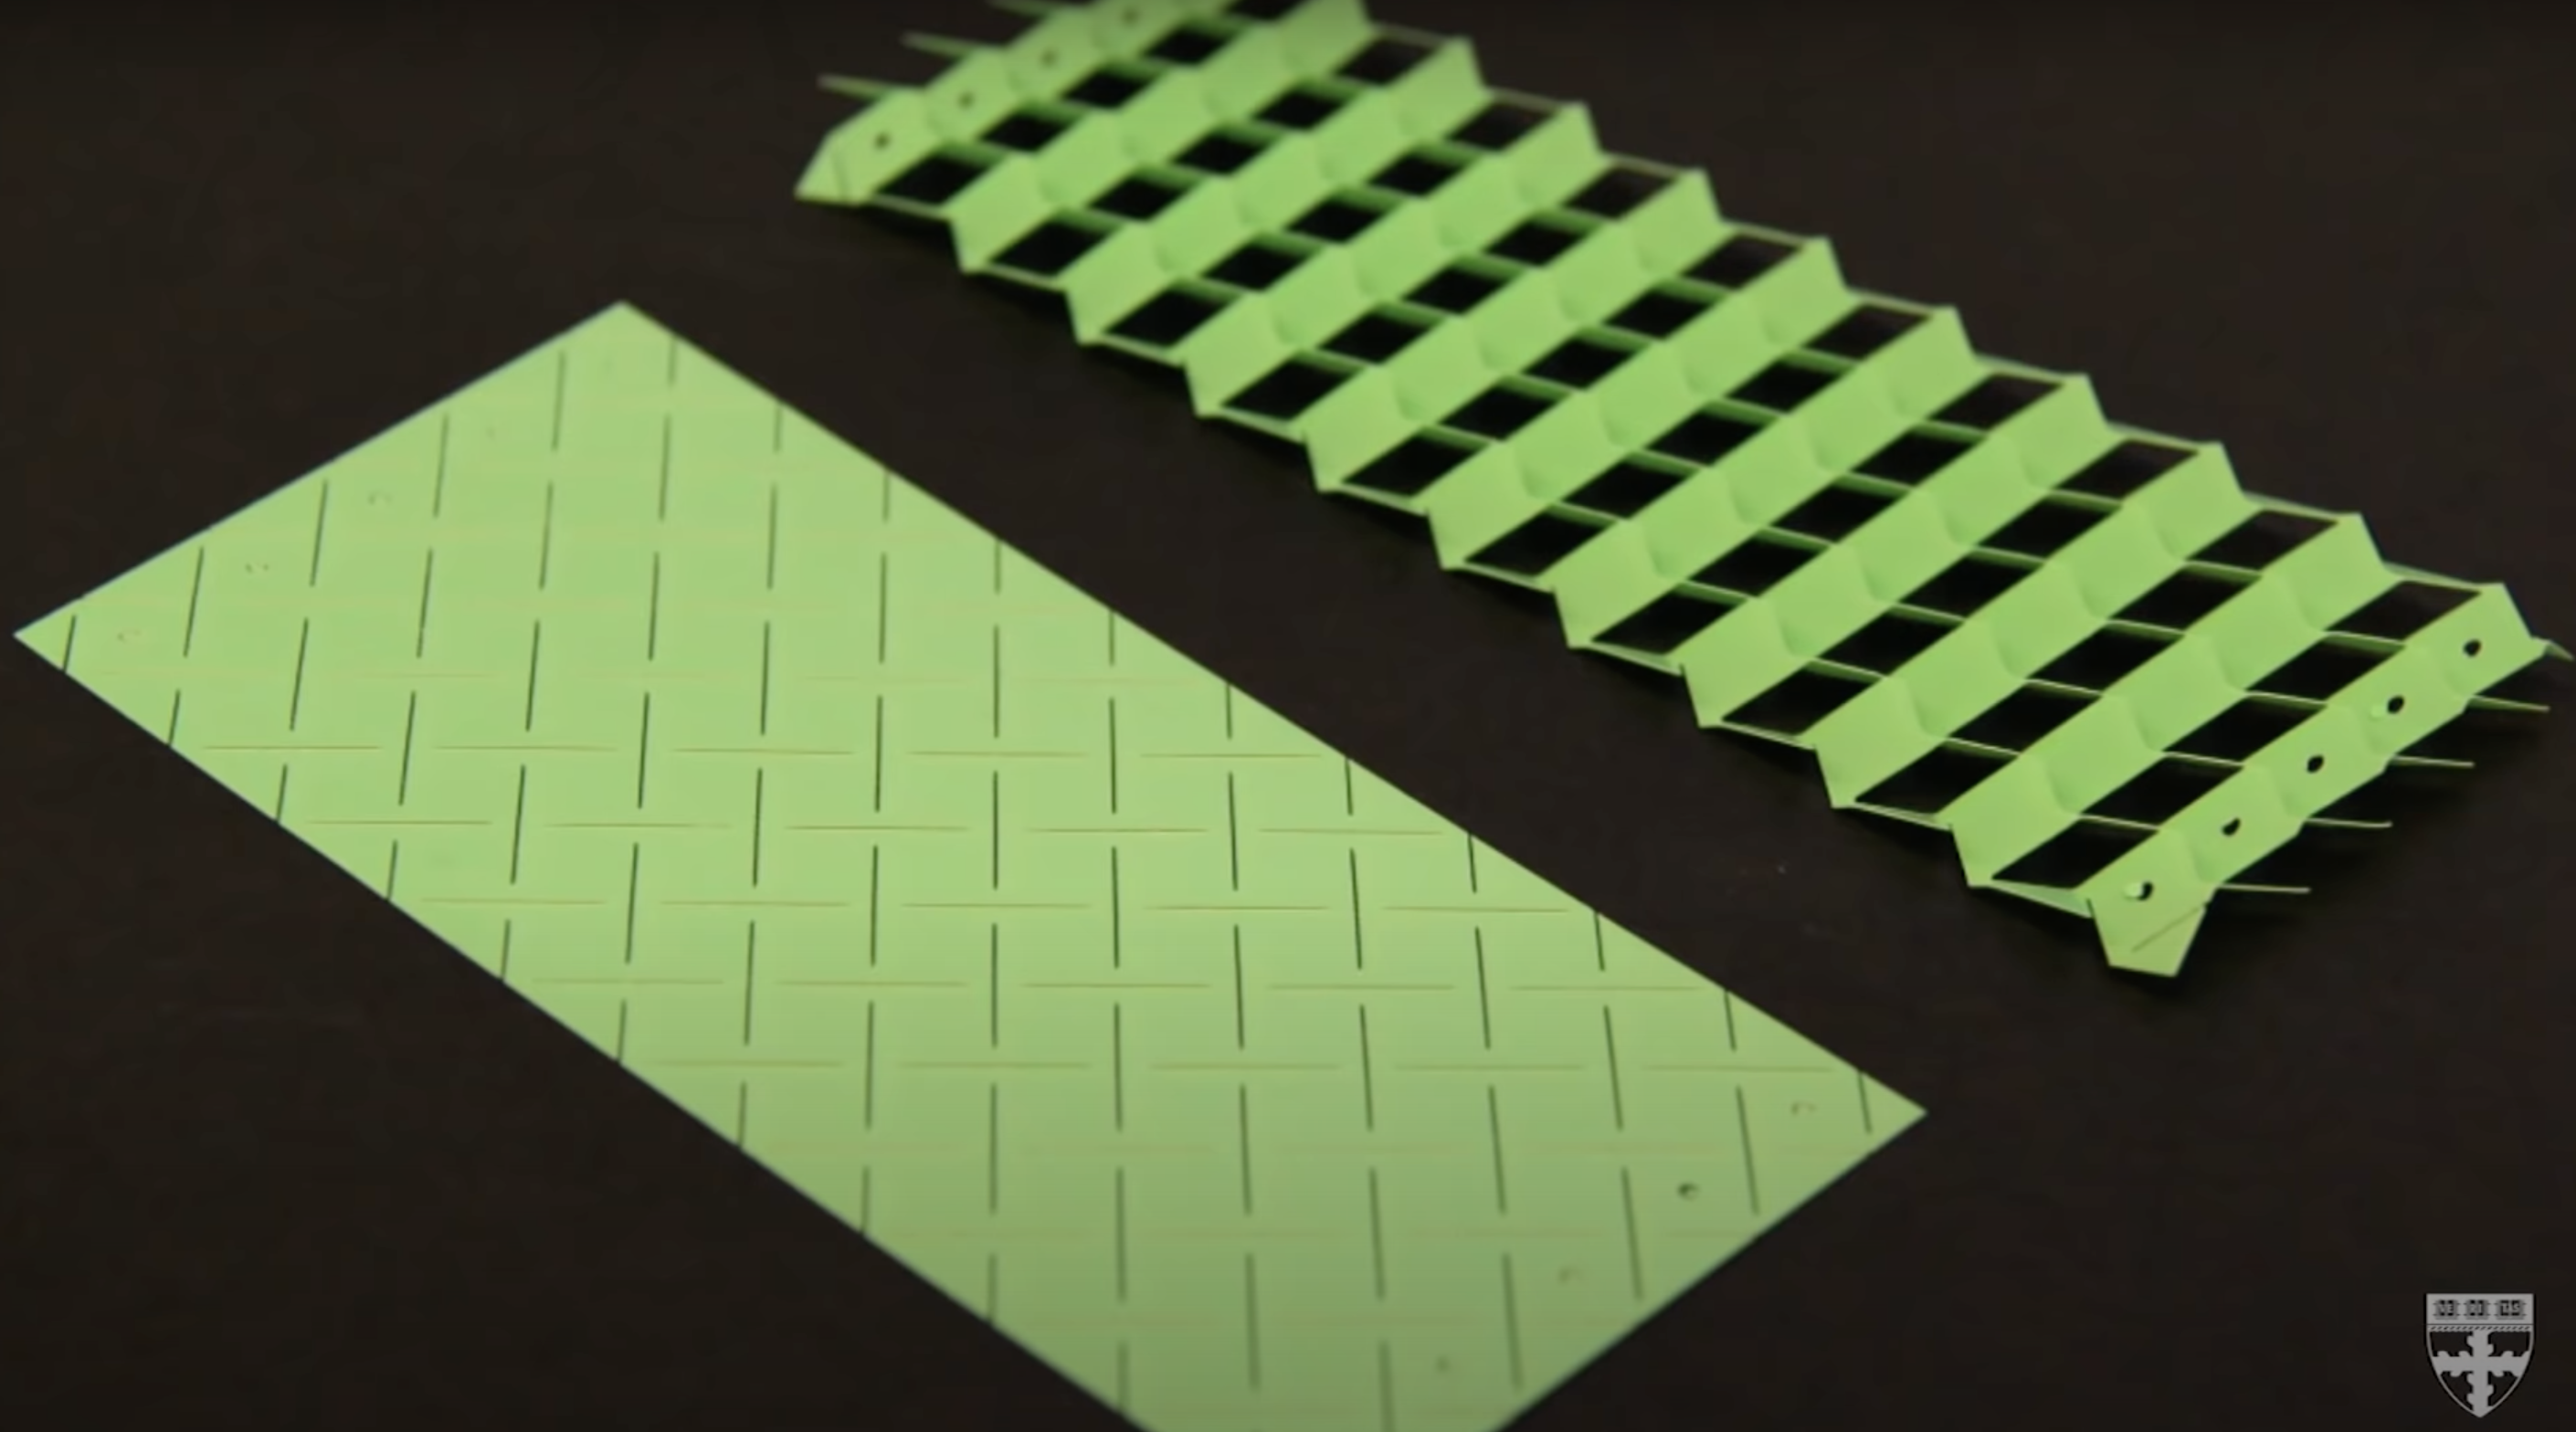
\includegraphics[height=0.6\textheight]{figures/kirigami_pattern_inspiration.png}
		\caption{New pop-up strategy inspired by cuts, not folds - Leah Burrows, Harvard John A. Paulson School of Engineering and Applied Sciences.}
	\end{figure}	
\end{frame}


\begin{frame}
	\frametitle{Stage 1 - Sheet Kirigami}
	\framesubtitle{Choosing a cut pattern}

	\begin{figure}
		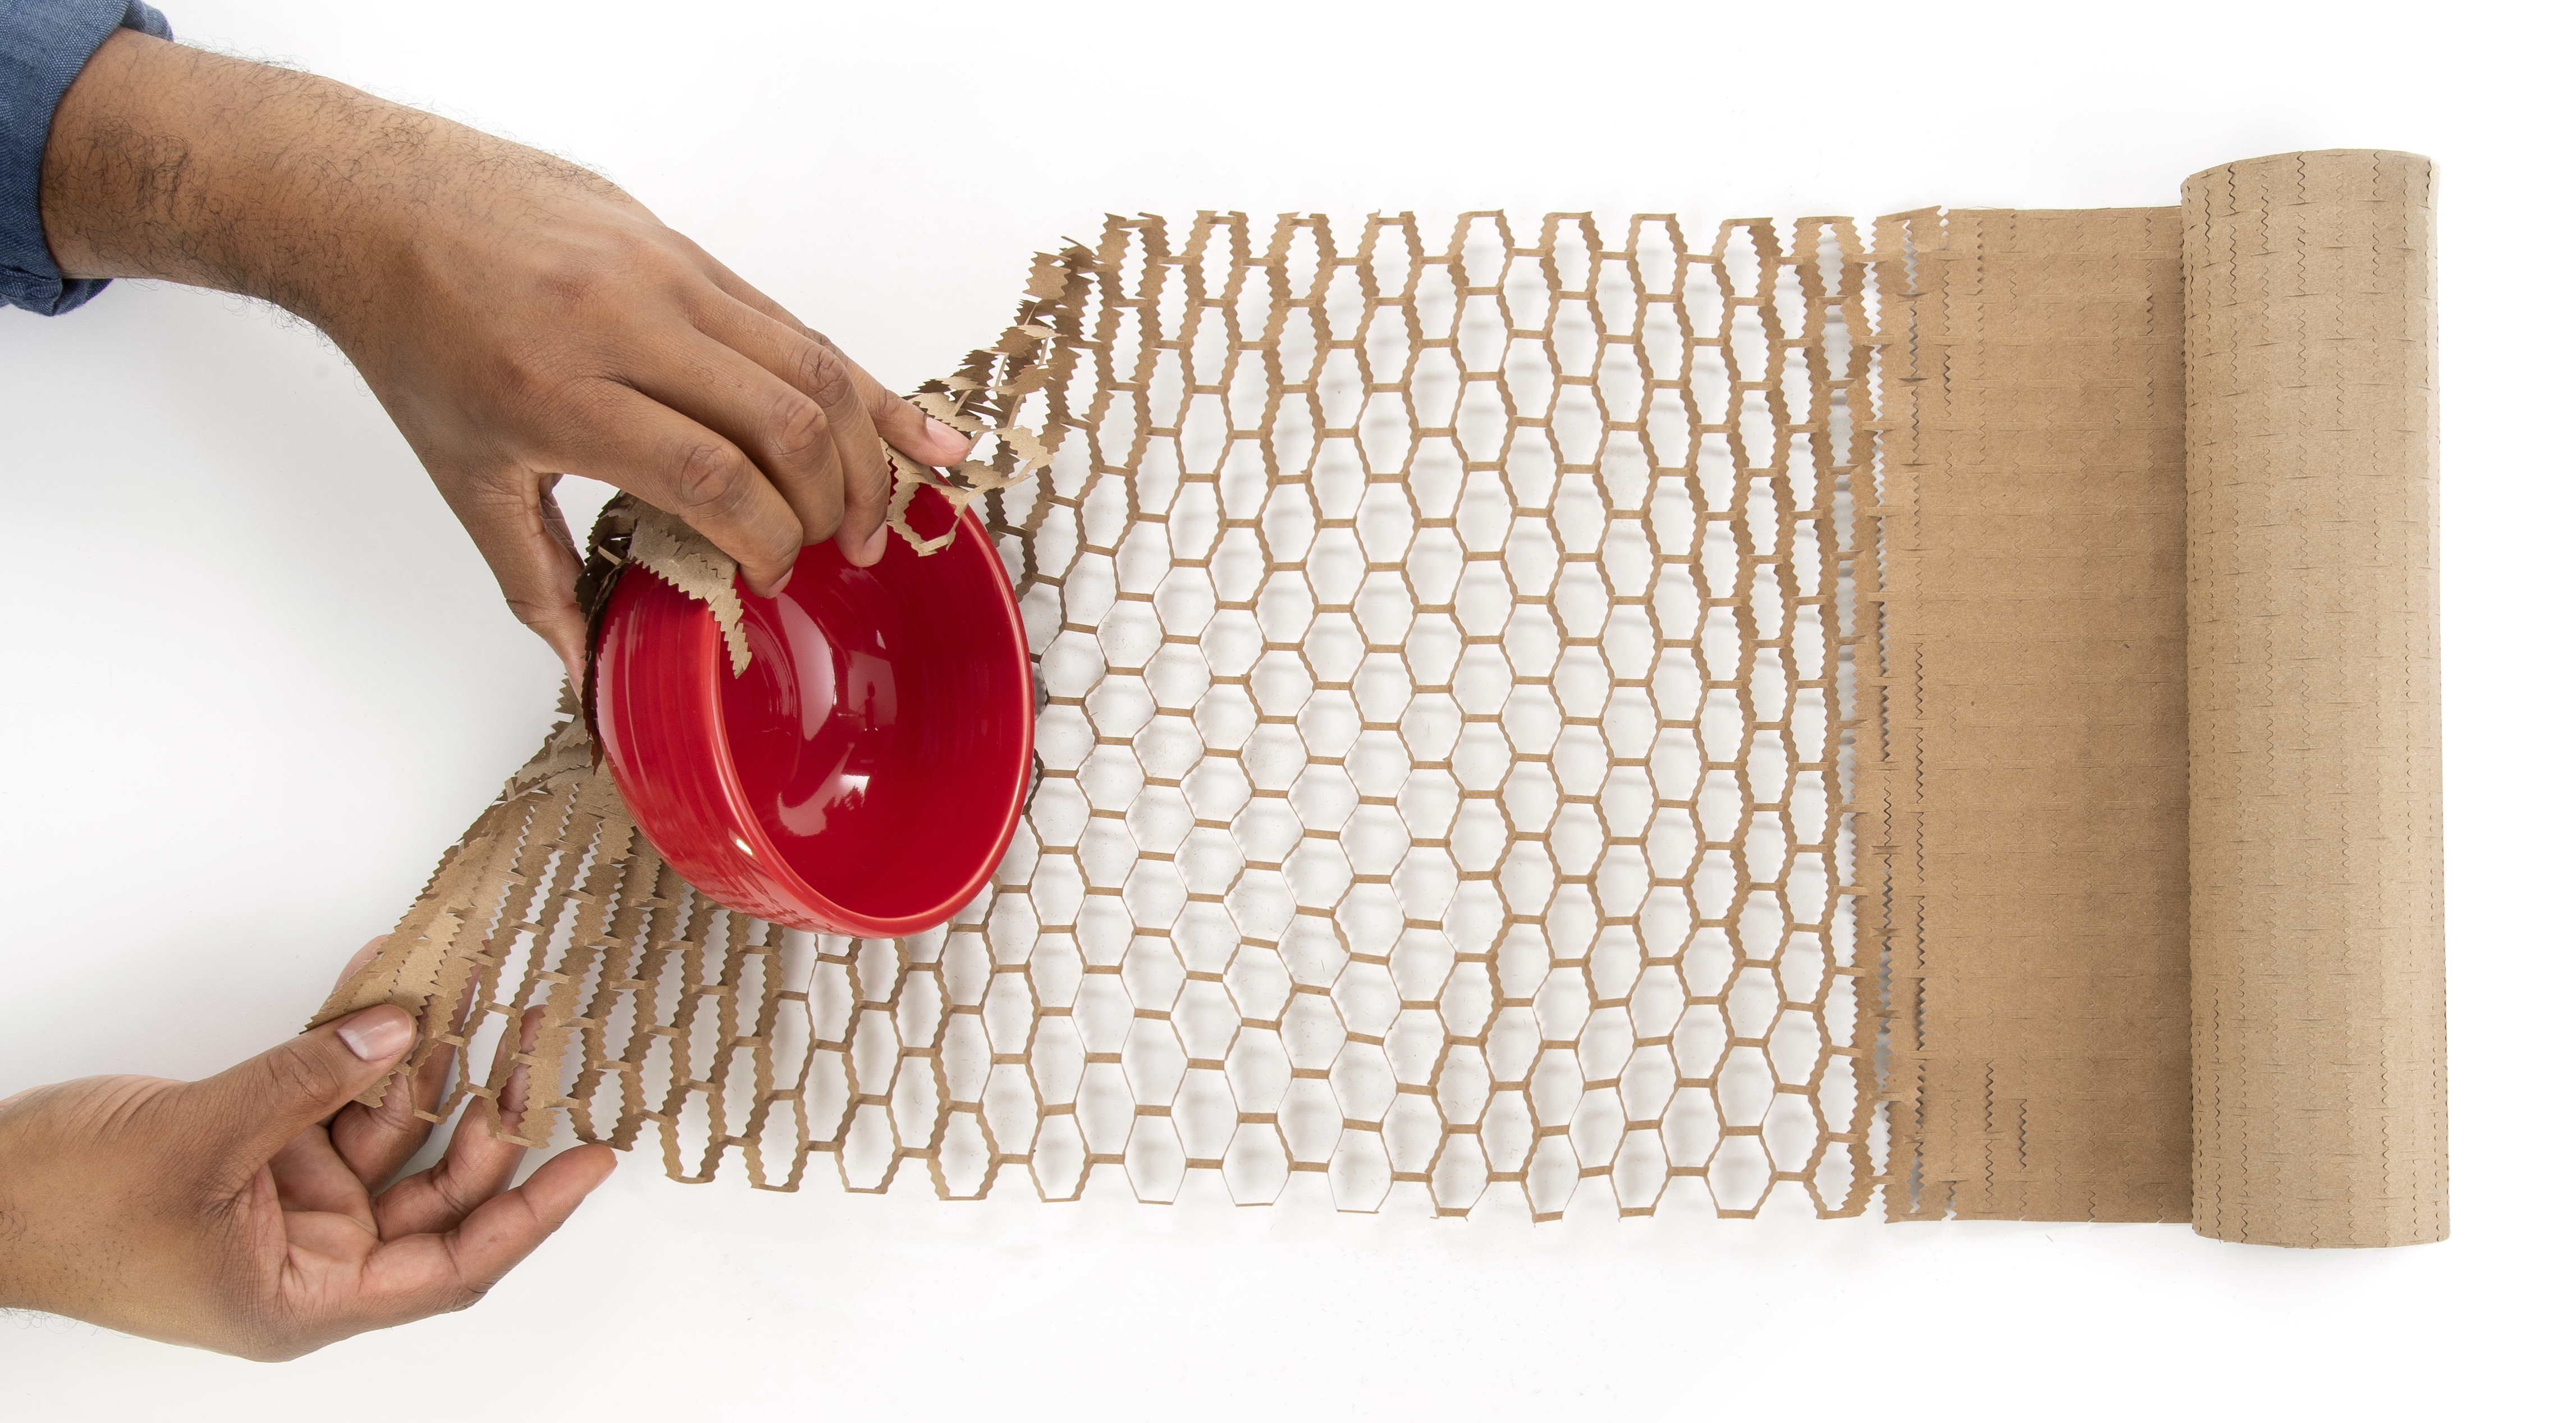
\includegraphics[height=0.6\textheight]{figures/Scotch_Cushion_Lock_1.jpg}
		\caption{Scotch Cushion Lock Protective Wrap.}
	\end{figure}	
	
\end{frame}



\begin{frame}
	\frametitle{Stage 1 - Sheet Kirigami}
	\framesubtitle{Implementation}

	% The Atomic Simulation Environment (ASE)

	\begin{figure}
		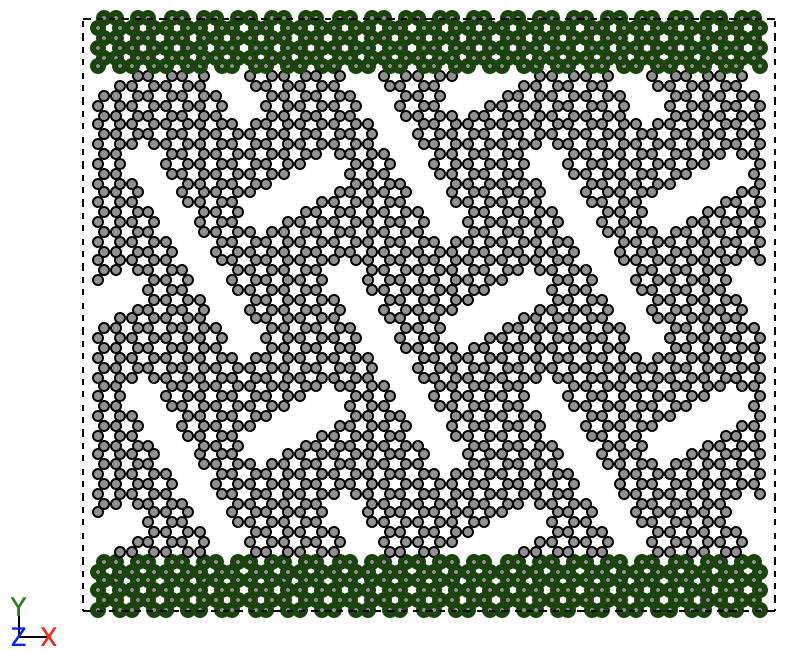
\includegraphics[height=0.6\textheight]{figures/cutpattern.png}
		\caption{Example of ``popup'' cut pattern. Grey color marks the cuttable sheet while green marks added blocks for stretching and dragging the sheet.}
	\end{figure}	

\end{frame}


\begin{frame}
	\frametitle{Stage 1 - Sheet Kirigami}
	\framesubtitle{Investigating 3D buckling}
	\begin{figure}
		\centering    
		\movie[open]{
\includegraphics[height=0.7\textheight, keepaspectratio]{figures/vacuum_stretch.png}}{figures/vacuum_stretch.mov}
		\caption{Kirigami sheet stretch in vaccuum.}
	\end{figure} 
\end{frame}


% \begin{frame}
% 	\frametitle{Stage 1 - Sheet Kirigami}
% 	\framesubtitle{Investigating 3D buckling}
% 	\begin{figure}
% 		\centering    
% 		\movie[open]{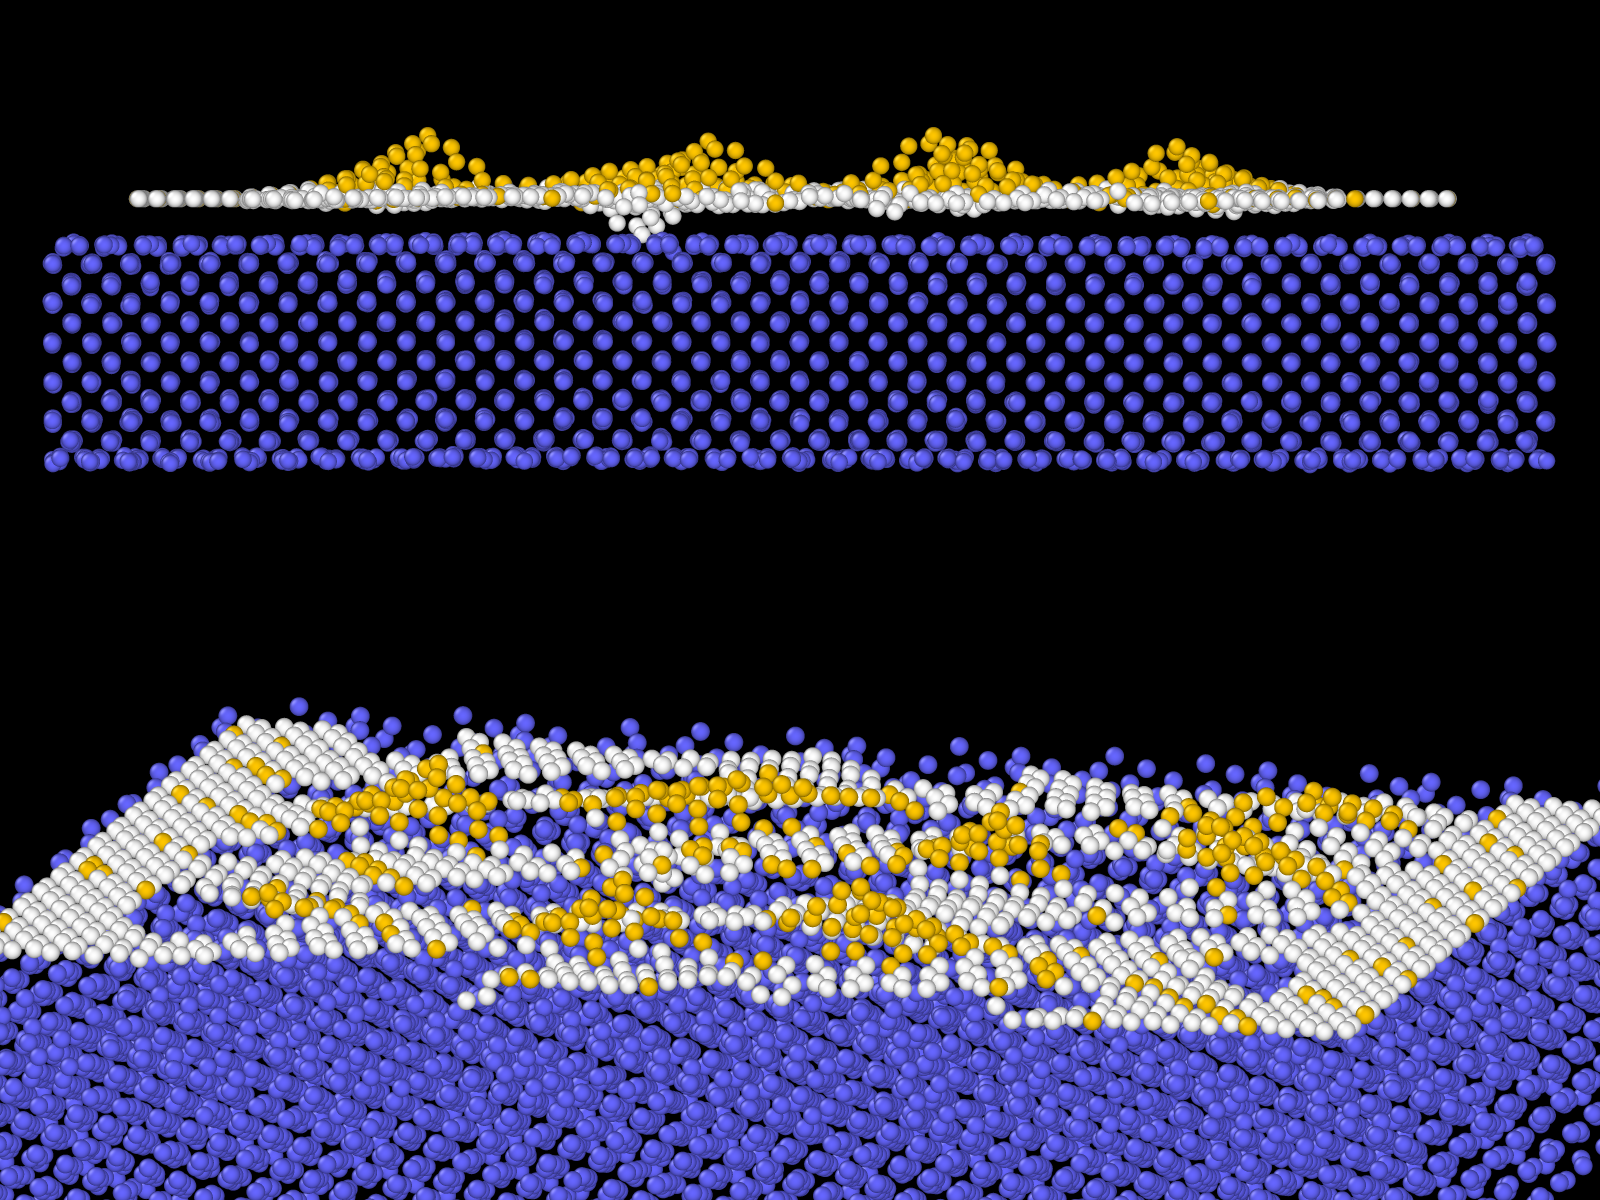
\includegraphics[height=0.7\textheight, keepaspectratio]{figures/contact_stretch.png}}{figures/contact_stretch.mov}
% 		\caption{Kirigami stretch in contact with Si-substrate.}
% 	\end{figure} 
% \end{frame}


% \begin{frame}
% 	\frametitle{Stage 1 - Sheet Kirigami}
% 	\framesubtitle{Investigating 3D buckling}
% 	\begin{figure}
% 		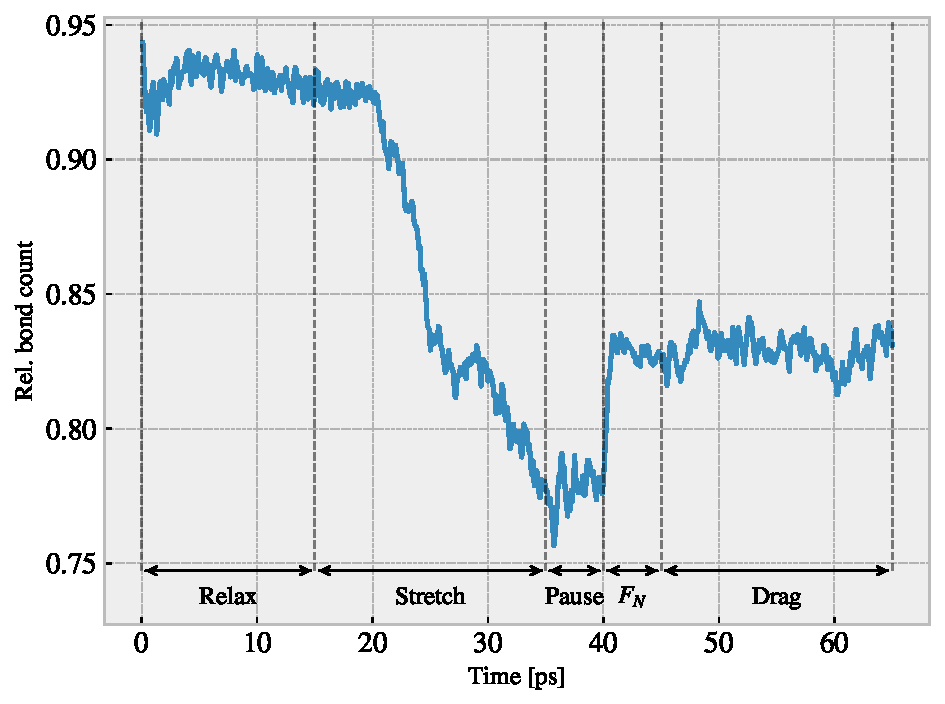
\includegraphics[height=0.7\textheight]{figures/contact_pct.pdf}
% 		\caption{Contact area approximation: Number of C-Si bonds within a threshold distance of 110\% the LJ interaction equilibrium distance.}
% 	\end{figure}	
% \end{frame}


\begin{frame}
	\frametitle{Stage 2 - Forward Simulation}
	\framesubtitle{Contact vs.\,Stretch}
	\begin{figure}
		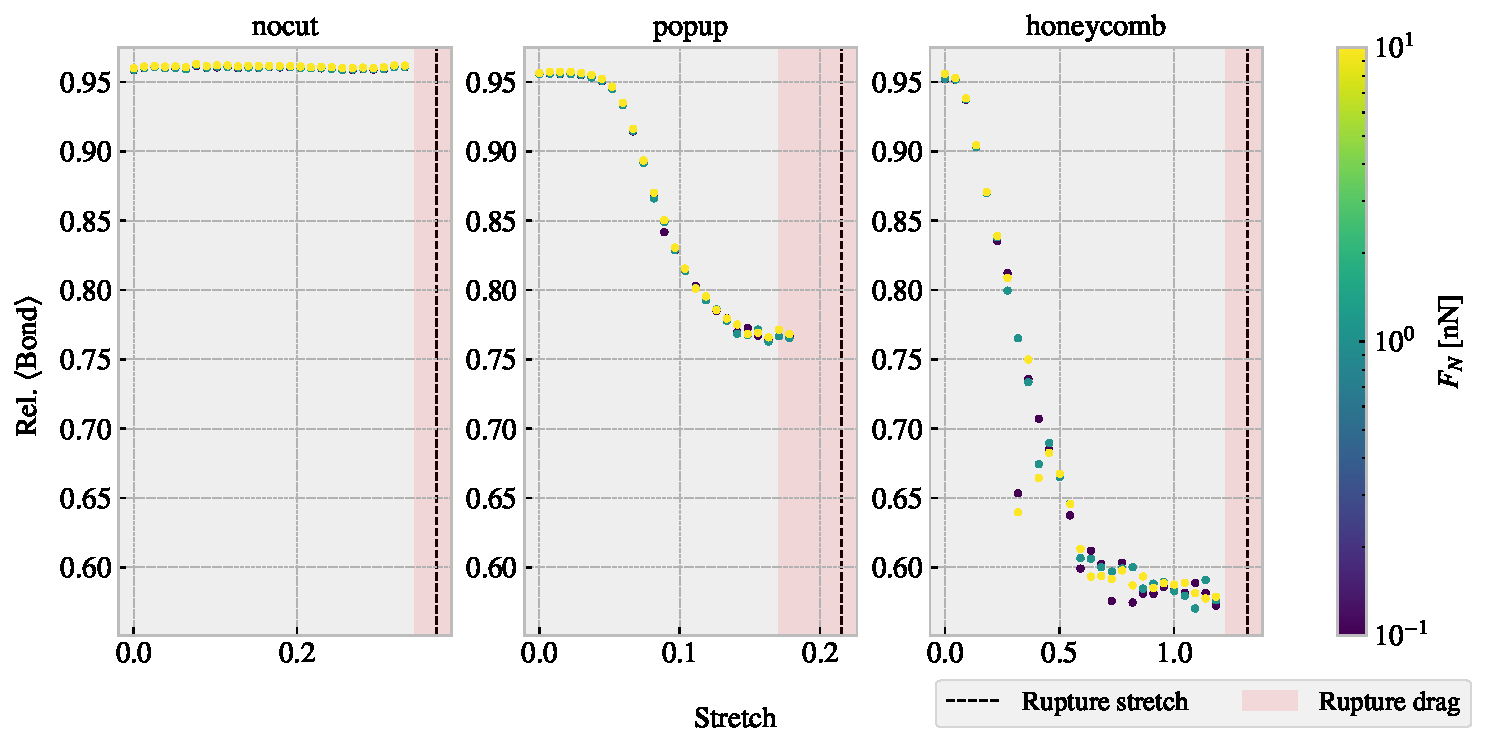
\includegraphics[height=0.65\textheight]{figures/multi_stretch_area_compare.pdf}
		\caption{Average relative amount of bonds between sheet and substrate as a function of stretch for different cut configurations.}
	\end{figure}	
\end{frame}

\begin{frame}
	\frametitle{Stage 2 - Forward Simulation}
	\framesubtitle{Friction vs.\,Stretch}
	\begin{figure}
		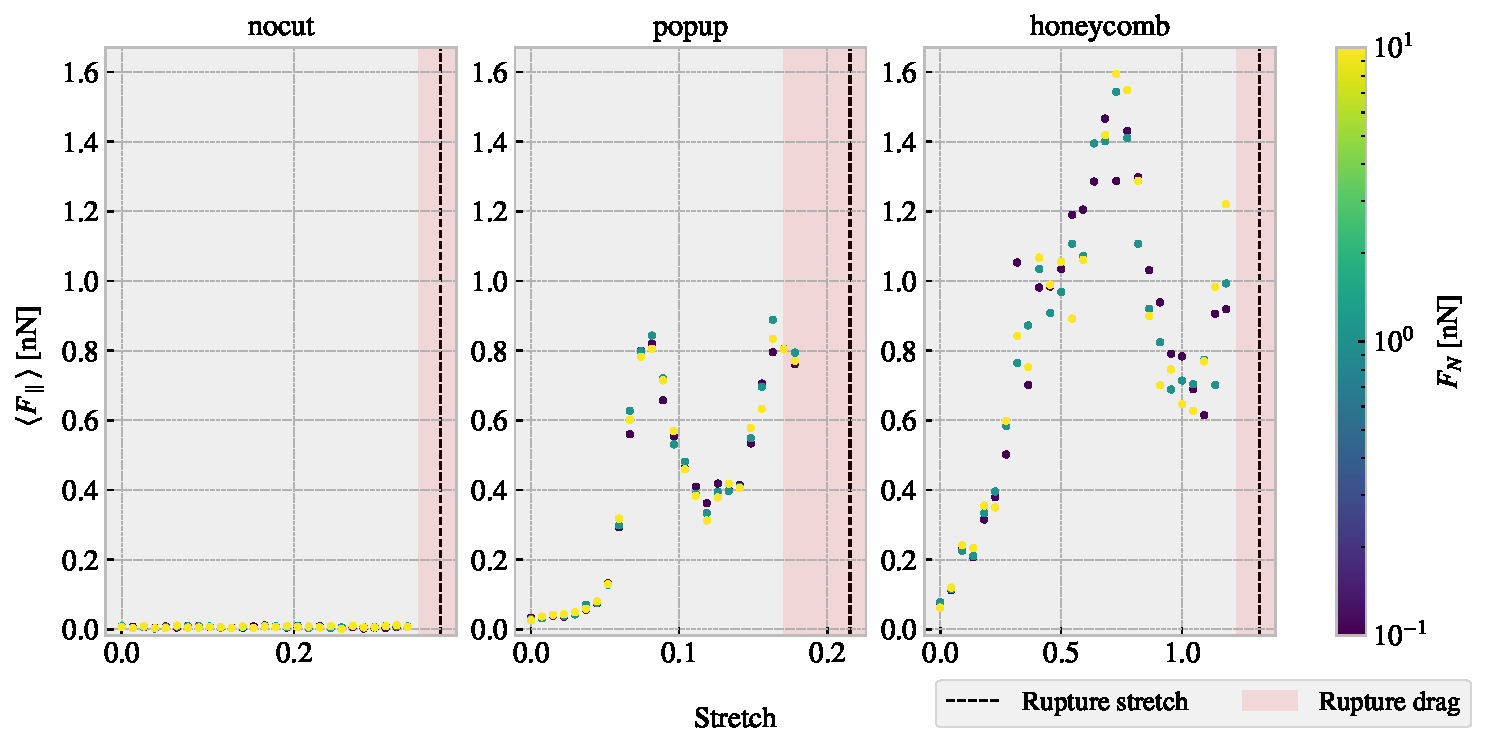
\includegraphics[height=0.65\textheight]{figures/multi_stretch_mean_compare.pdf}
		\caption{Mean friction force $F_{\parallel}$ parallel to drag direction as a function of stretch of the sheet for different cut configurations.}
	\end{figure}	
\end{frame}


\begin{frame}
	\frametitle{(Stage 4 - Nanomachine applications) }
	\framesubtitle{Negative friction coefficient}

	\begin{align*}
		\left.\begin{aligned}
			\text{Normal force} &: F_f = k \cdot F_N \\
			\text{Stretch} &: F_f \sim s \cdot \text{stretch}  \\
			\text{Nanomachine}&: \text{stretch} = \pm R \cdot F_n
		  \end{aligned}\right\} \Longrightarrow F_f \propto \underbrace{(k \pm sR)}_{\mu} \cdot F_n
	\end{align*}
	
	\begin{figure}
		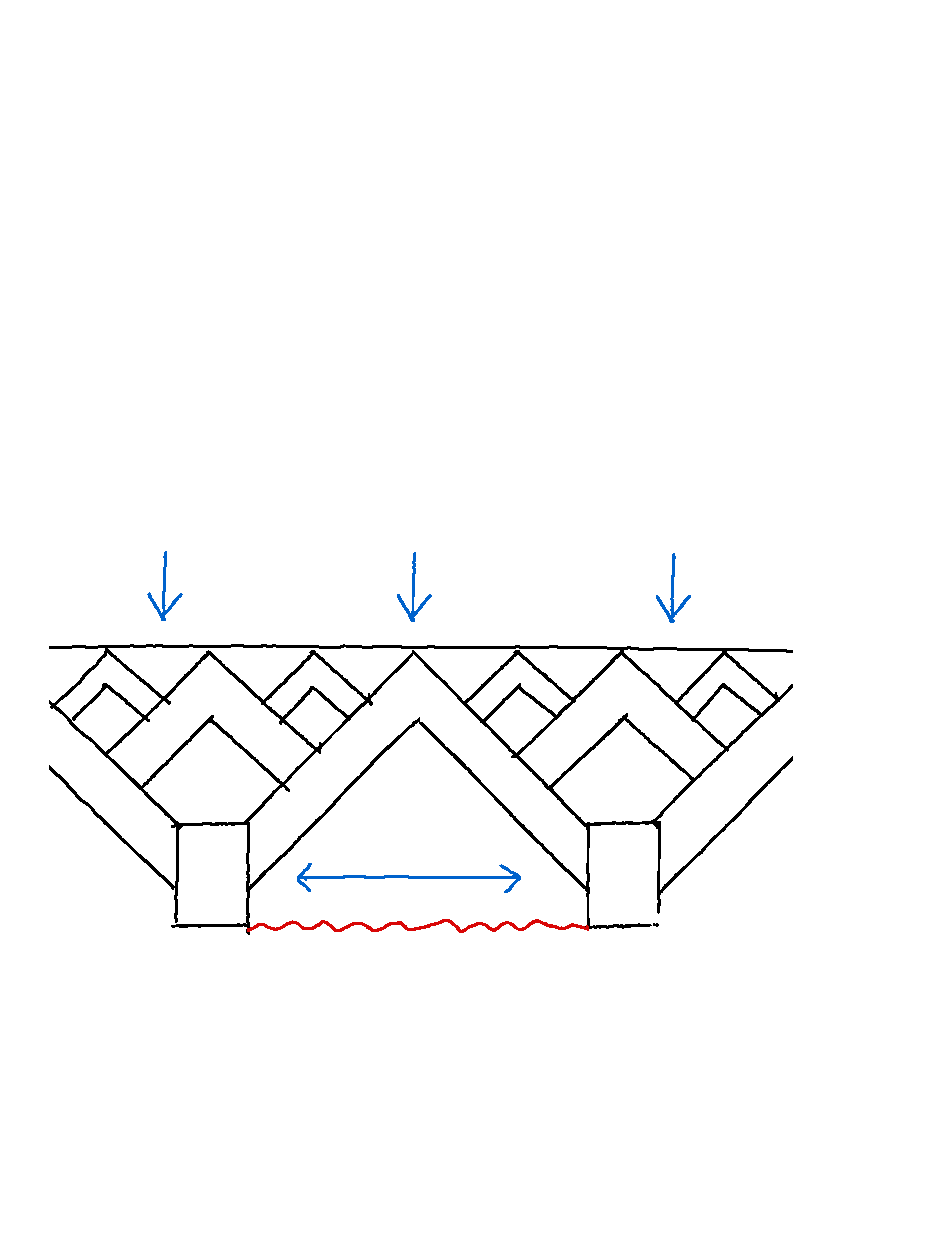
\includegraphics[width=0.6\linewidth]{figures/nanomachine.pdf}
		\caption{Sketch for nanomachine coupling normal force and stretch. Black represents nanomachine components and red the sheet.}
	\end{figure}	
	
\end{frame}



\begin{frame}
	\frametitle{Stage 3 - Inverse design}
	\framesubtitle{Inverse design}
	\textit{Designing complex architectured materials with generative adversarial networks, YUNWEI MAO, 2020.}
	\begin{figure}
		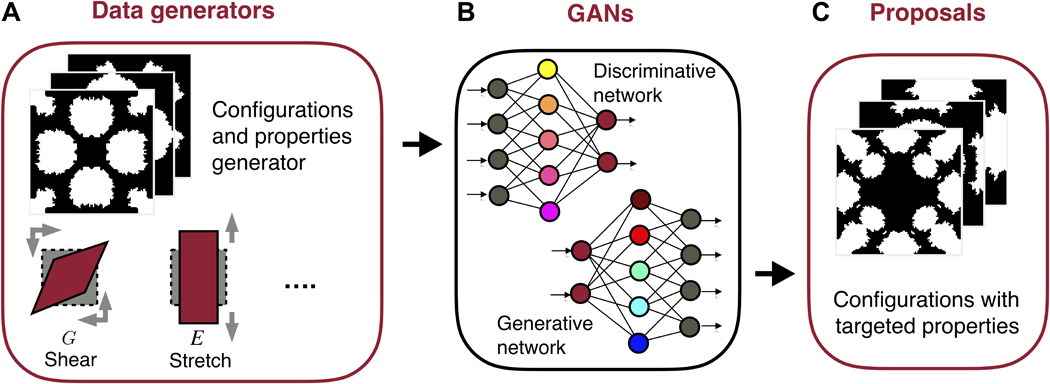
\includegraphics[width=0.8\linewidth]{figures/ML_procedure.jpeg}
		\caption{(A) Data generators to generate datasets of configurations and properties of architectured materials. (B) GANs trained by the datasets. (C) New designs of architectured materials with the targeted properties proposed by the GANs.}
	\end{figure}
\end{frame}


\begin{frame}
	\frametitle{Interpretation of PhD project}
	\framesubtitle{}

	{\large Topic and methods}
	\begin{itemize}
		\item Alpine mass movements and cascading processes
		\item Multi-phase material point method (MPM)
	\end{itemize}
	\vspace*{7px}
	
	{\large Tasks}
	\begin{itemize}
		\item Writing high performance code for solvers and data analysis
		\item Benchmarking different implementations
		% First step: Two-phase hydromechanical MPM with solid and fluid phases
	 	% Second step: Introduce heat energy balance equation (friction heat, dissipation and phase changes)
		\begin{itemize}
			\item Melting block of ice
			\item Sliding on 3D-printed topography
			\item Avalanches on test sites
			\item Previous disasters
		\end{itemize}
	\end{itemize}
	\vspace*{7px}
	
	
	{\large Development expectations}
	\begin{itemize}
		\item Gain knowledge of snow and granular mechanics
		\item Gain knowledge of MPM method
		\item Build strong academic and social connections
		\item Experience the lifestyle of an alpine environment
	\end{itemize}

	

	


	% {\Large Steps}
	% \begin{enumerate}
	% 	\item Two-phase hydromechanical MPM in which solid and fluid phases
	% 	\item Introduce heat energy balance equation (friction heat, dissipation and phase changes)
	% 	\item Benchmarking
	% \end{enumerate}
	% \vspace*{20px}




	% In modeling, one major difficulty is the combined numerical description of processes such as multi-phase interactions, heat transfer, phase changes, and  liquefaction during the flow.

	
\end{frame}




\end{document} 


